\subsection{Predstavitev stroja in kosa}
Za svoj stroj sem si izbral dolgo-stružni avtomat Gauthier GM-127. 
Ima 5 držal za orodja in 2 gnana orodja, vidnih na spodnji 
sliki \ref{gauthier_priblizano}. Omogoča struženje do ø12 
mm. Ima tudi možnost nadgradnje z roko za preprijem kosa in 
povrtavanje iz druge strani.

\begin{figure}[H]
    \begin{center}
        \includegraphics[width=8cm]{gauthier_slika.jpg}
        \caption{Slika stroja, katerega sem nastavljal
        \cite{interna}}
        \label{gauthier_priblizano}
    \end{center}
\end{figure}

Za izdelek, sem si izbral končnik žice iz materjala 1.4305.
Spodaj levo na sliki \ref{delavniska_risba} je delavniška risba z 
merami in tolerancami kosa, desno pa je 3D model izdelka v izometričnem 
pogledu, narejen v programu Blender.

\begin{multicols}{2}
    \begin{figure}[H]
        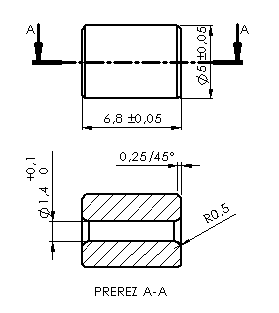
\includegraphics[width=\linewidth]{izdelek_risba.png}
        \caption{Risba končnika žice
        \cite{interna}}
        \label{delavniska_risba}
    \end{figure}

    \columnbreak

    \begin{figure}[H]
        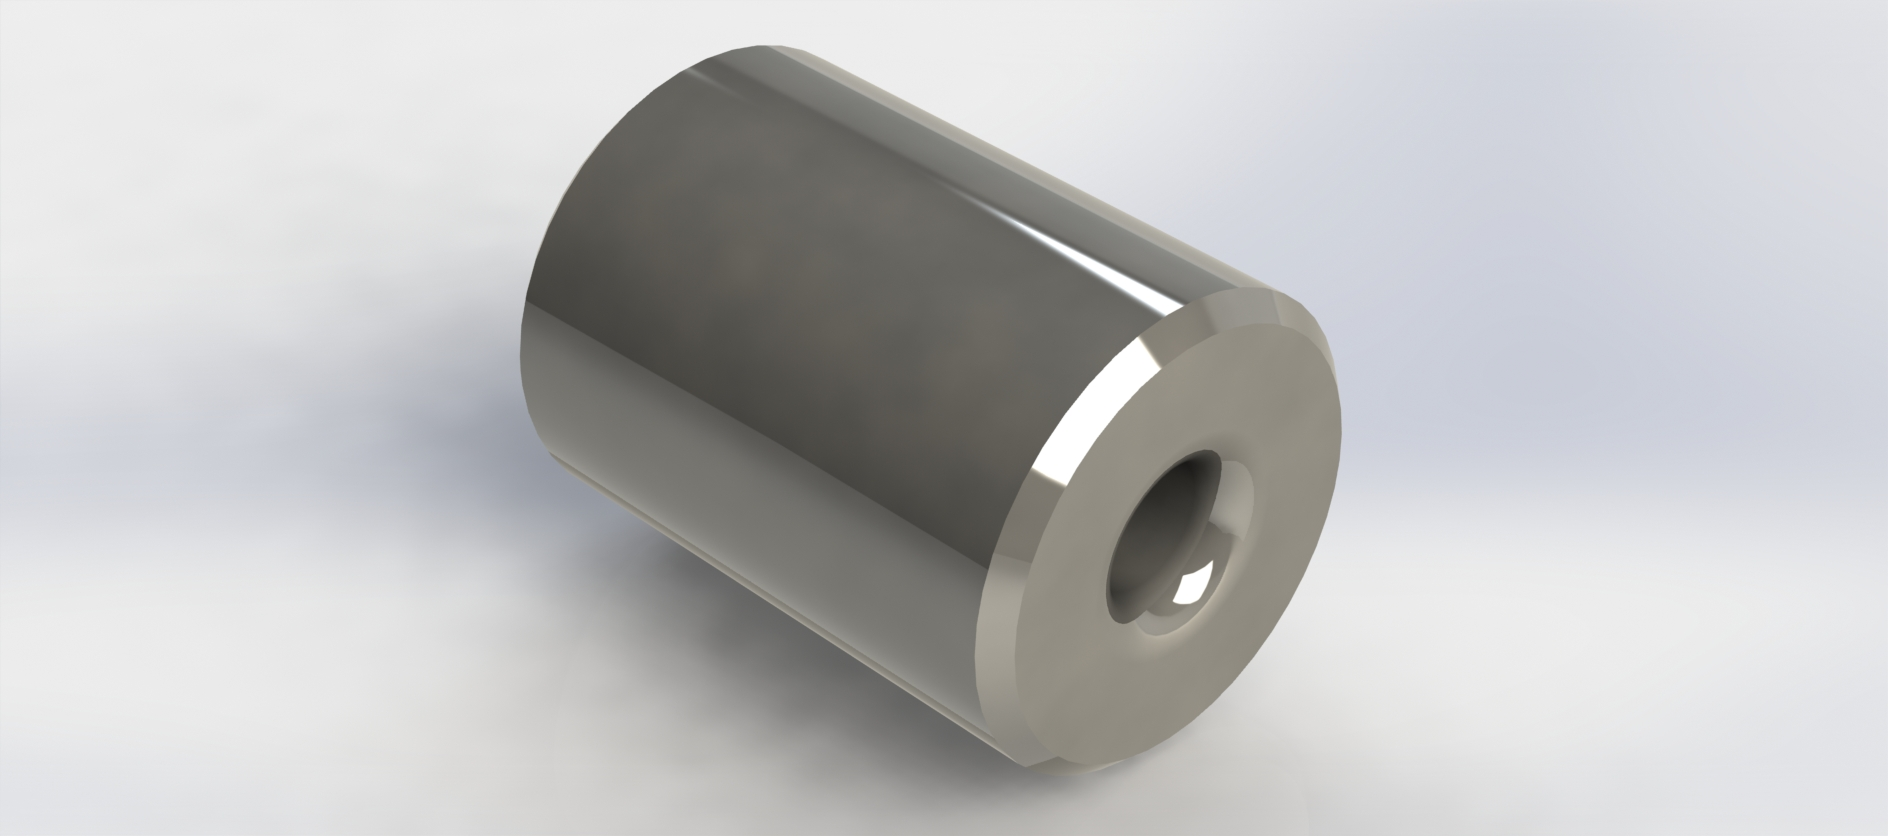
\includegraphics[width=\linewidth]{izdelek_cad.jpg}
        \caption{3D model izdelka
        \cite{lasten}}
        \label{3d_model}
    \end{figure}
\end{multicols}

\newpage